\subsection{Protocollo di comunicazione}
In generale, il protocollo di comunicazione prevede che il client invii messaggi di comando in cui venga specificato il tipo di comando da eseguire, il server, ricevuto e letto il comando, lo esegue e invia un messaggio di risposta.\\
Ogni comando prevede un trasferimento file, quindi, a seconda del tipo di comando, o nel messaggio di comando o in quello di risposta viene allegato il file, con le informazioni necessarie alla sua corretta ricezione.\\
Ogni messaggio di comando e di risposta è composto da campi di un numero fissato di byte contenenti le informazioni necessarie all'interpretazione del messaggio.
Essendo un'applicazione distribuita, i campi vengono distinti utilizzando variabili la cui ampiezza (numero di bit) è indipendente dall'architettura della macchina, a tal proposito ogni campo informativo è composto dalle variabili definite in \emph{stdint.h}, ad esempio un campo di 8 bit è rappresentato da una variabile di tipo \emph{uint8\_t}.\\ 
I primi 8 bit di un messaggio di comando indicano sempre il tipo di comando da eseguire e, a seconda del comando, possono avere o meno ulteriori informazioni.

\begin{lstlisting}[title=Costanti comandi]
// command codes
#define LIST 		0
#define GET 		1
#define PUT 		2

// response codes
#define GET_OK      0
#define GET_NOENT   1
#define PUT_SUCCESS 2
#define PUT_FAILURE 3
\end{lstlisting}

%\begin{figure}
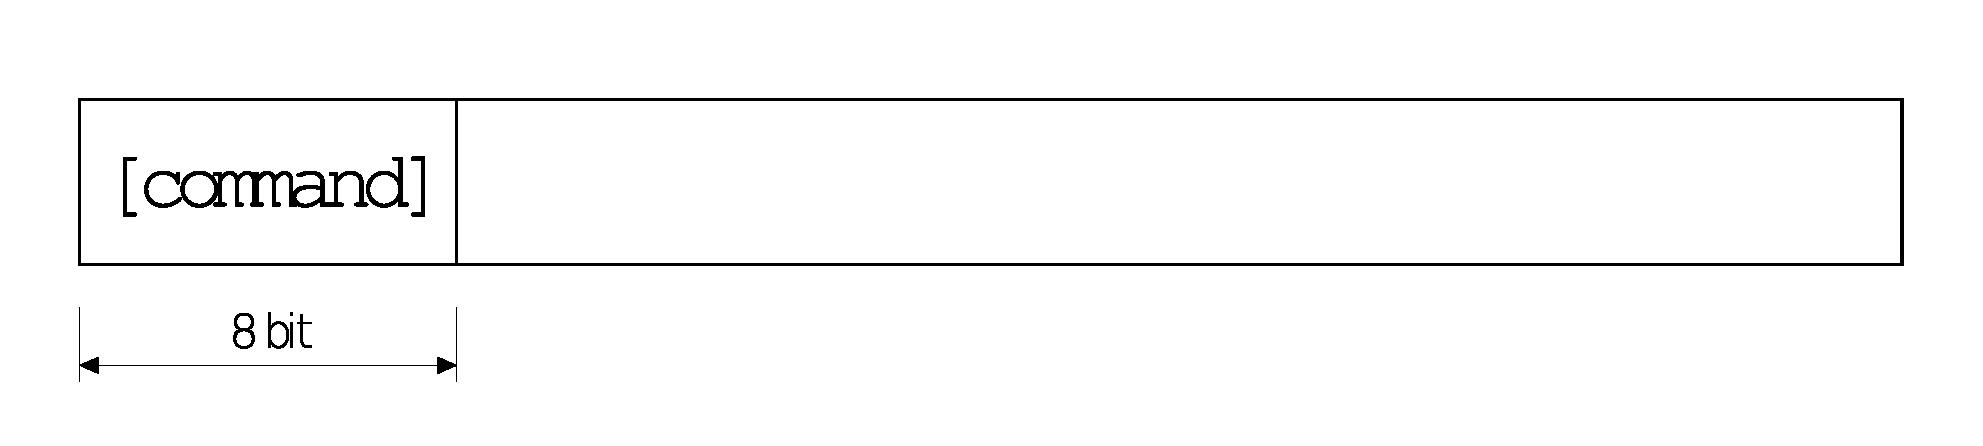
\includegraphics[scale=0.35]{images/gen_message}
%\end{figure}

Una volta impostati i vari campi in un buffer, se non va inviato un file, i dati vengono passati direttamente al livello di trasporto virtuale.\\
Se altrimenti, va inviato un file, viene chiamata la funzione \emph{send\_file}, i campi informativi vengono considerati un header per il file ed il tutto viene frammentato (per non allocare troppa RAM) e passato al livello sottostante.\\
Lato opposto il ricevente analizza uno alla volta i campi informativi, poi legge il file tramite la funzione \emph{recv\_file}.\\
Uno dei parametri necessari alla ricezione di un file è quello relativo alla dimensione dello stesso,
che corrisponde ad un campo di 8 byte. Ciò implica che esiste un limite superiore, seppur molto ampio,
relativo alla dimensione dei file che si possono inviare pari a $2^{64} - 1$ byte.\\
L'arternativa sarebbe stata quella di usare una variabile a 32 bit, ma si sarebbe avuto un limite inferiore ai 4 GiB,
leggermente limitante per un'applicazione FTP.

\begin{lstlisting}[title=cmd\_commons.c]
void send_file(int fd, void *header, size_t file_size, 
				size_t header_size)								
{                                                                                                       
	int8_t buffer[MAX_BUFSIZE];                                                                         
	size_t buf_size, total_size;                                                                        
	unsigned int i, n;                                                                                  
																										
	total_size = header_size + file_size;                                                               
	n = total_size / MAX_BUFSIZE;                                                                       
																										
	memcpy(buffer, header, header_size);                                                                
																										
	for (i = 0; i <= n; i++) {                                                                          
																										
		// calculate last bytes to send                                         
		if (i == n) {           
			buf_size = total_size % MAX_BUFSIZE;                                                        
			if (!buf_size)                                                                              
				// total size is a multiple of MAX_BUFSIZE:
				// send only n-1 chunks        
				break;          
		} else                                                                                          
			buf_size = MAX_BUFSIZE;                                                                     
																										
		if (readn(fd, buffer + header_size, buf_size - header_size)
			== -1)                              
			handle_error("readn() - reading file to send");

		header_size = 0;  // consider header only at the first pass

		rdt_send(buffer, buf_size);
	}
}

void recv_file(int fd, size_t size)
{
	unsigned int i, n = size / MAX_BUFSIZE;
	size_t buf_size;
	int8_t buffer[MAX_BUFSIZE];
                                                                                              
	for (i = 0; i <= n; i++) {
                                                                                              
		// calculate last bytes to store 
		if (i == n) {           
			buf_size = size % MAX_BUFSIZE;
			if (!buf_size)
				// size is a multiple of MAX_BUFSIZE:
				// receive only n-1 chunks
				break;          
		} else
			buf_size = MAX_BUFSIZE;
                                                                                              
		rdt_recv(buffer, buf_size);
                                                                                              
		if (writen(fd, buffer, buf_size) == -1)
			handle_error("writen() - writing received file");
	}
}
\end{lstlisting}

\subsubsection{Comando LIST}

Nel messaggio di comando list non sono previsti campi aggiuntivi oltre a quello che specifica il comando.

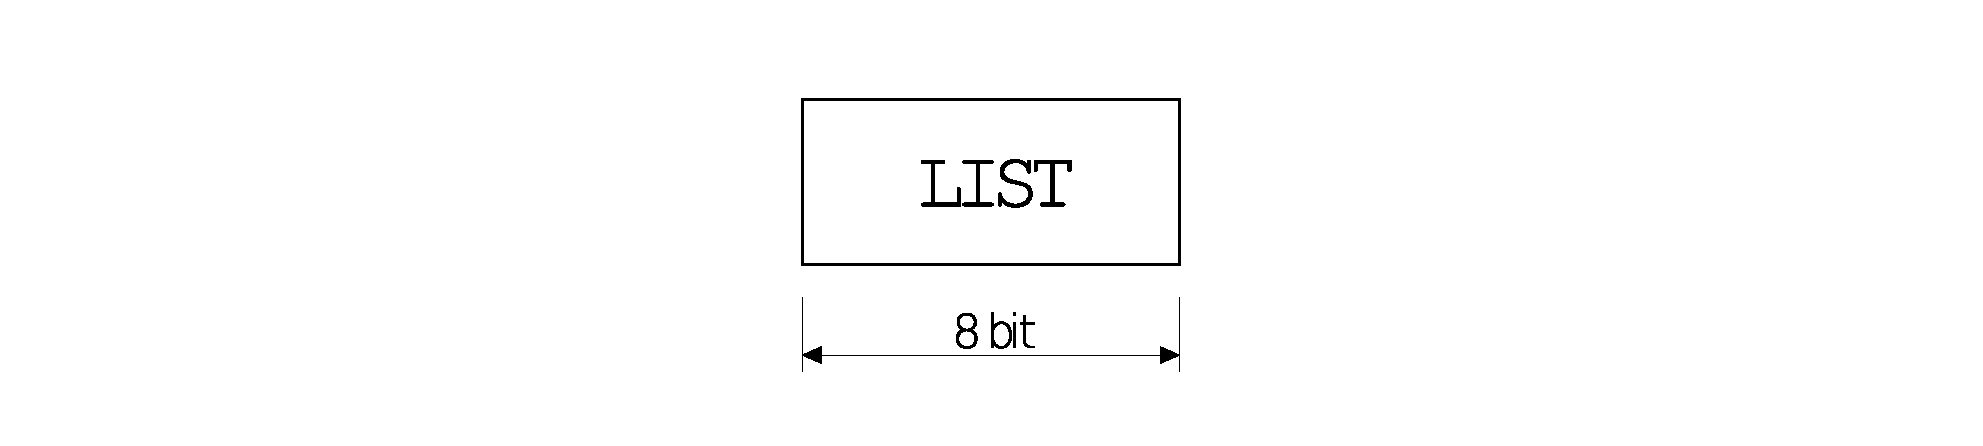
\includegraphics[scale=0.35]{images/list_client}

Il server ricevuto il comando, esegue il comando di sistema \emph{ls} redirigendo l'output sul file \emph{file\_list.txt}, dopodiché viene impostato il messaggio di risposta con la dimensione del file (campo da 64 bit) e a seguire il file contenente la lista dei file disponibili al download.

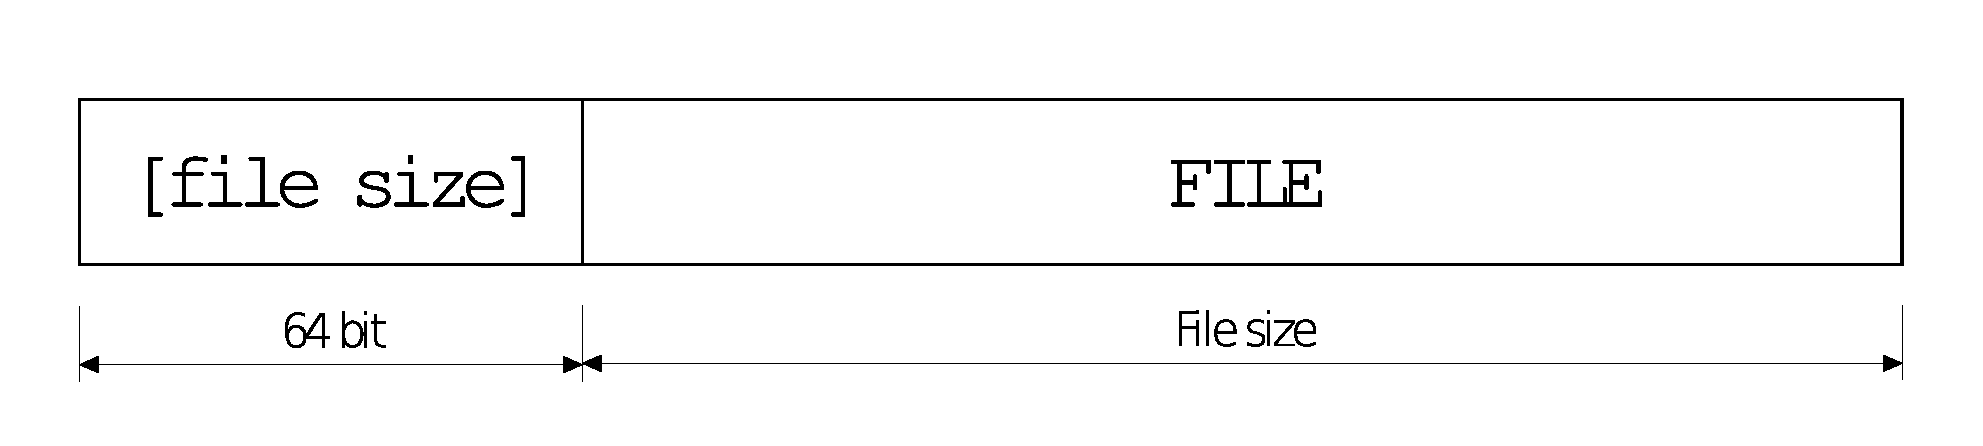
\includegraphics[scale=0.35]{images/list_server}

\begin{lstlisting}[title=clicmd.c]
void cli_list()
{
    uint8_t cmd = LIST;
    uint64_t file_size;
    char *buffer;

    /* send LIST command */
    rdt_send(&cmd, sizeof(cmd));

    /* read list size */
    rdt_recv(&file_size, sizeof(file_size));

    /* allocate buffer */
    buffer = malloc(file_size);
    if (!buffer)
        handle_error("malloc()");

    /* recv file list */
    rdt_recv(buffer, file_size);

    /* print file list and free memory */
    printf("\n%s\n", buffer);
    free(buffer);
}                                                                
\end{lstlisting}

\begin{lstlisting}[title=srvcmd.c]
void srv_list(void)
{
    int fd;
    struct stat st;
    uint64_t file_size;
    uint8_t *header;
    char *filename = "file_list.txt";

    /* execute ls command */
    char *cmd = "ls > file_list.txt";
    if (system(cmd) == -1)
        handle_error("system() - executing ls command");

    /* open the destination file of the list command */
    fd = open(filename, O_RDONLY);
    if (fd == -1)
        handle_error("open() - opening LIST file");

    /* calculate file size */
    if (fstat(fd, &st) == -1)
        handle_error("fstat() - getting LIST file stats");
    file_size = st.st_size;

    /* allocate header buffer */
    header = malloc(sizeof(file_size));
    if (!header)
        handle_error("malloc() - allocating LIST header");

    /* set the header */
    memcpy(header, &file_size, sizeof(file_size));

    /* send file and free resources */
    send_file(fd, header, file_size, sizeof(file_size));
    free(header);
    if (close(fd) == -1)
        handle_error("close() - closing file list");
}
\end{lstlisting}

\subsection{Comando GET}
Nel messaggio di comando get, i primi 8 bit che specificano il comando sono seguiti dal nome del file che si vuole scaricare, questo campo è composto da un numero indefinito di byte, il server lo interpreta come una stringa, pertanto legge fintanto che non trova il terminatore di stringa.

%	+-------+-----------------------+
%	|  GET  |	   file_name     	|
%	+-------+-----------------------+
%  	  8 bit

Il server una volta ottenuto il nome del file, controlla se è presente in memoria e, in caso affermativo, prepara il messaggio di risposta così strutturato:
i primi 8 bit contengono una costante che indica che il file esiste, i successivi 64 bit la dimensione del file, infine segue l'intero file.

%+---------+-------------------------+---------------------------+
%| GET_OK  |	       file_size        |	..		file		..	|
%+---------+-------------------------+---------------------------+
%  8 bit				64 bit
	
Se il file non esiste, viene inviato un messaggio di soli 8 bit contente la costante che ne indica l'assenza.

%+-----------+
%| GET_NOENT |
%+-----------+
%  	8 bit

\subsubsection{Comando PUT}
Nel messaggio di comando put, dopo i primi 8 bit che specificano il comando, segue il nome del file delimitato dal terminatore di stringa, la dimensione del file in un campo di 64 bit ed infine il file stesso.

	%+-------+-----------------------+---------------------------+-----------------------------------+
	%|  PUT  |	   file_name     	|		  file_size         |	..			file			..	|
	%+-------+-----------------------+---------------------------+-----------------------------------+
	%  8 bit										64 bit

Il server avvia la procedura di ricezione al termine della quale invia indietro un messaggio di 8 bit con l'esito dell'operazione.

	%+-----------+							+-----------+
    %|PUT_SUCCESS|         oppure            |PUT_FAILURE|
    %+-----------+                           +-----------+
	%	8 bit									8 bit

